\documentclass[
11pt,]{beamer}
\usepackage{booktabs}
%\graphicspath{{Images/}{./}}
\usetheme{Antibes}
\usefonttheme{default}
\usepackage{palatino} 
\usepackage[default]{opensans}
\useinnertheme{circles}
\usepackage[english,russian]{babel}

\setbeamertemplate{caption}{\raggedright\insertcaption\par}

\usepackage{graphicx} % подключение графики
\usepackage{pdfpages} % вставка pdf-страниц
\usepackage{amsmath} % дополнительные математические возможности
\usepackage{amssymb} % дополнительные математические символы
\usepackage{physics}
\usepackage{tikz}
\usetikzlibrary{decorations.markings}
\usepackage{subcaption}
\usepackage{pgfplots}
\usepgfplotslibrary{
	groupplots,
}

\usepackage{adjustbox}



\newcommand{\average}[1]{\langle #1 \rangle}
\newcommand{\tderiv}[1]{\cfrac{d #1}{d t}}
\newcommand{\deriv}[2]{\frac{\partial #1}{\partial #2}}
\newcommand{\cderiv}[2]{\cfrac{\partial #1}{\partial #2}}

\newcommand{\avarage}[1]{\left\langle #1 \right\rangle}


\title{Термализация неупругой тёмной материи в Солнце} 
\author[]{Товстун А.А.}
\institute[shortinst]{ИЯИ РАН}

\begin{document}	
	\begin{frame}
		\titlepage % Output the title slide, automatically created using the text entered in the PRESENTATION INFORMATION block above
		{
			\centering
			\textit{QFTHEP-270} \\
			\par
		}
	\end{frame}
	
%	\begin{frame}
%		\frametitle{WIMP}
%		\begin{itemize}
	\item WIMP (массивные слабовзаимодействующие частицы), один из кандидатов на тёмную материю.
	\item для термального рождения Тёмная Материя должена иметь сечение аннигилляции $$\average{\sigma_{ann} v} \sim 10^{26} \text{см}^3\text{с}^{-1}
	$$
	\item Методы поиска: прямые (подземные эксперименты по поиску отдачи ядер), косвенные (измерение продуктов аннигиляции), коллайдерные.
\end{itemize}
%	\end{frame}
	
	\begin{frame}
		\frametitle{Термальная темная материя (WIMP)}
		\begin{itemize}
	\item Поиски тёмной материи сильно ограничивают сечение рассеяние на нуклоне.
\end{itemize}

\begin{figure}
	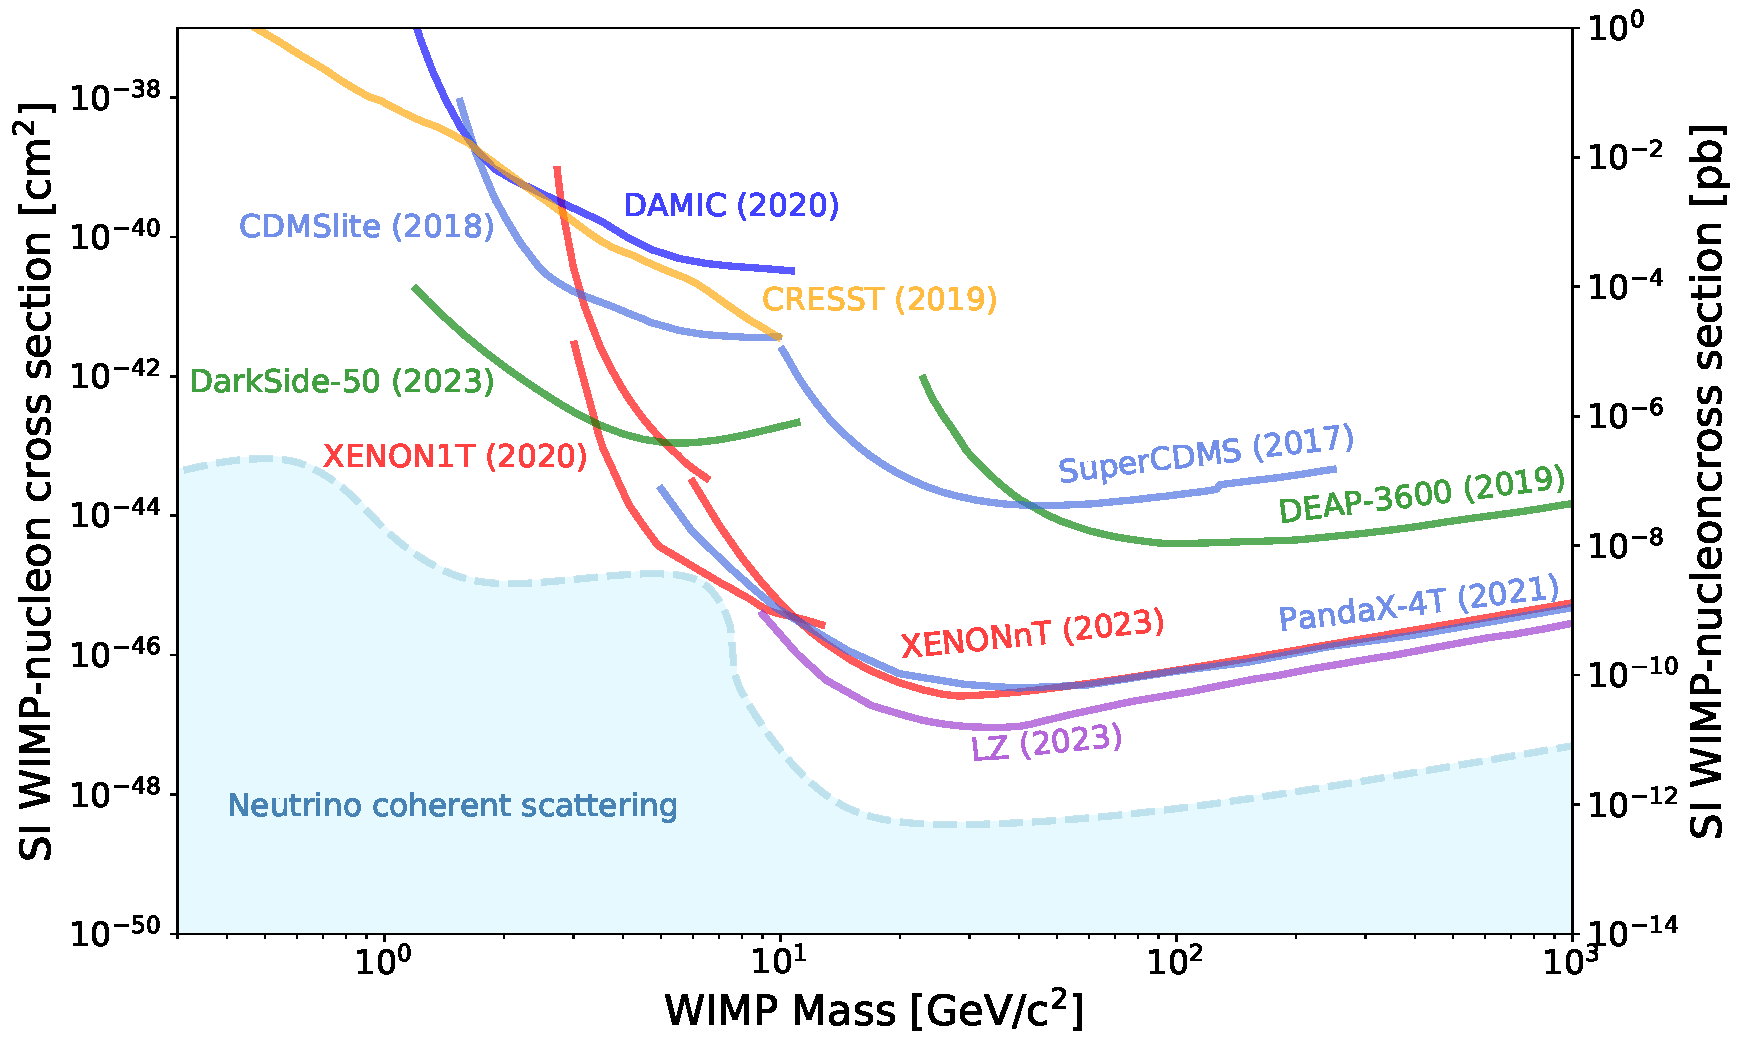
\includegraphics[width=0.53\textwidth]{images/pdg_si_limits.pdf}
	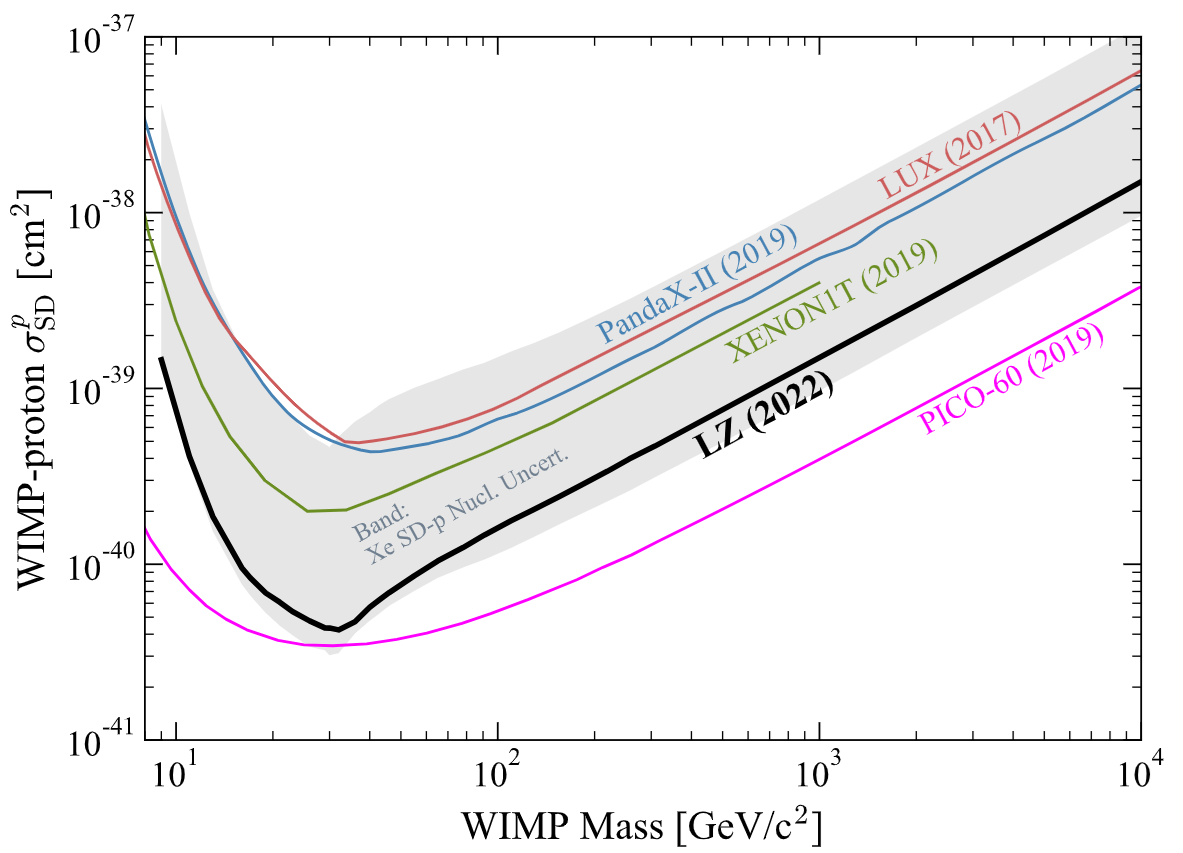
\includegraphics[width=0.45\textwidth]{images/DirectSD.png}
	\caption{Ограничения на спин-независимое сечение ТМ на нуклоне $\sigma^{SI}_{\chi p}$ \footnote{PDG, DarkMatter} и спин-зависимое $\sigma^{SD}_{\chi p}$ \footnote{arXiv:2410.23454}}
\end{figure}

	\end{frame}
	
	\begin{frame}
		\frametitle{Неупругая тёмная материя}
		\begin{itemize}
	\item Неупругая тёмная материя позволяет ослабить ограничения благодаря кинематике.
	\item Состоит из 2 компонент: $\chi$ с массой $m_{\chi}$ и $\chi^*$ с массой $m_{\chi}+ \delta$
	\item Столкновения с ядрами происходят преимущественно неупругим образом.
	
	\begin{center}
		\begin{tikzpicture}[line width=1pt, scale=1.2,fermion/.style={postaction={decorate},decoration={markings, mark=at position 0.5 with {\arrow{>}}}}]
			% Define vertices
			\node at (0, 1) (chi_in) {\(\chi, k\)};
			\node at (0, -1) (N_in) {\(N, p\)};
			\node at (3, 1) (chi_out) {\(\chi^*, k'\)};
			\node at (3, -1) (N_out) {\(N, p'\)};
			\node[circle, fill=black, inner sep=1.5pt,outer sep=0pt] at (1.5, 0) (vertex) {};
			
			\node[left] at (-1, 0) {\(N + \chi(m)\)};
			\node[right] at (4, 0) {\(N + \chi^*(m + \delta)\)};
			% Draw arrows for incoming and outgoing particles
			\draw[fermion] (chi_in) -- (vertex)  node[midway, above ] {};
			\draw[fermion] (N_in) -- (vertex) node[midway, below ] {};
			\draw[fermion] (vertex) -- (chi_out) node[midway, above ] {};
			\draw[fermion] (vertex) -- (N_out) node[midway, below ] {};
		\end{tikzpicture}
	\end{center}
\end{itemize}
	\end{frame}
	
	\begin{frame}
		\frametitle{Пример модели неупругой тёмной материи.}
		Неупругая тёмная материя может естественно возникать в различных теориях.
\begin{itemize}
	\item Простейший пример --- дираковский фермиона малой майорановской массой
	\begin{equation*}
		\mathcal{L}_{kin} \supset \overline{\chi}( i\gamma^{\mu} \partial_{\mu} - m)\chi + 
		\frac{\delta}{4} \overline{\chi} \chi^C + \frac{\delta}{4} \overline{\chi^C} \chi %+\frac{1}{2} m_2 \bar{\psi} \gamma^5 \psi^C 
	\end{equation*}
	Массовыми состояниями являются 
	\begin{eqnarray*}
		\chi_1 = \cfrac{\chi - \chi^C}{\sqrt{2} i} 
		%+O(\frac{\delta}{m_{\chi}})
		,\chi_2 = \cfrac{\chi+ \chi^C}{\sqrt{2}}
		%  + O(\frac{\delta}{m_{\chi}})
	\end{eqnarray*}
	с массами $m_1 = m - \frac{\delta}{2}$ и  $m_2 = m + \frac{\delta}{2}$
\end{itemize}
	\end{frame}
	
	\begin{frame}
		\frametitle{Пример модели неупругой тёмной материи.}
		\begin{itemize}
	\item В простейшем случае рассмотрим векторное взаимодействие, которое приводит к неупругому рассеянию.
	\begin{equation*} 
		\mathcal{L} \supset g\bar{\chi}\gamma^{\mu}\chi \bar{q}\gamma_{\mu}q = i\frac{g}{2}
		\left[ \bar{\chi_2}\gamma^{\mu}\chi_1  -  \bar{\chi_1}\gamma^{\mu}\chi_2\right]\bar{q}\gamma^{\mu}q
	\end{equation*}  
	\item Данный механизм встречается в секторе хиггсино в SUSY расширениях и в некоторых моделях с тёмными фотонами.
	\item Похожий механизм со скалярными комплексными полями встречается в секторе снейтрино.
\end{itemize}
	\end{frame}
	
	
	\begin{frame}
		\frametitle{Тёмная материя в Солнце}
		\begin{itemize}
	\item Тёмная материя с $m_{\chi} \sim \text{GeV} -\text{TeV} $ может захватываться и аннигилировать в Солнце. Эти процессы описывают уравнением баланса (если пренебречь испарением)
	\begin{equation*}
		\tderiv{N(t)} = C - C_A N^2
	\end{equation*}
	решение которого имеет вид:
	\begin{equation*}
		N = \sqrt{\cfrac{C}{C_A}} \th{[\sqrt{C_A t^2C}]} \quad
		\Gamma(t) = \frac{1}{2} C \th^2{[\sqrt{C_A t^2C}]}
		\label{eq:AnnNtherm}
	\end{equation*}
 
\end{itemize}
	\end{frame}
	
	\begin{frame}
		\frametitle{Тёмная материя в Солнце}
		\begin{itemize}
	\item Зная зависимость темпа аннигилляции в конечный момент эволюции $T_{\odot}$ (время жизни Солнца) от скорости захвата :
	 \begin{equation*}
	 	\Gamma =  \cfrac{1}{2 C_A T_{\odot}^2} F(C_A T_{\odot}^2 C) \quad F(x) = x\th^2{\sqrt{x}}
	 \end{equation*}
	 можно сделать ограничения на $\sigma_{\chi p}$:
	 \begin{equation}
	 	\sigma_{\chi p} < \sigma_{\chi p, 0} \cfrac{1}{C_A T_{\odot}^2 \cdot C(\sigma_{\chi p,0})} F^{-1}\left(	2\Gamma_{max} \cdot C_A T_{\odot}^2\right)
	 \end{equation}
	\item  В упругом случае как правило $C_AT_{\odot}^2 C >> 1$ и $\Gamma = \frac{C}{2}$.
	\begin{equation}
		\sigma_{\chi p} < \sigma_{\chi p, 0} \cfrac{2\Gamma_{max}}{C(\sigma_{\chi p,0})} 
	\end{equation}
\end{itemize}
	\end{frame}
	
	\begin{frame}
		\frametitle{Тёмная материя в Солнце}
		\begin{itemize}
	\item В упругом случае как правило $aT_{\odot}^2C >> 1$ и $A = C$. 
	\item В неупругом сценарии $a$ зависит от сечения рассения $\sigma_{\chi p}$, модели и времени.
	\item Величина $a$ находится с помощью численного расчета линейного уравнения Больцмана.
	\item Учитывая изотропность задачи, фазовое пространство --- плоскость $E$ --- $L$ и уравнение эволюции выглядит следующим образом:
\end{itemize}

\begin{eqnarray*}
	\cderiv{f(E,L)}{t} = C(E,L) + \\
	 + \int{dE'dL' [S(E,L,E',L') f(E',L') - S(E',L',E,L)f(E,L)]}
\end{eqnarray*}

	\end{frame}

	
	\begin{frame}
	\frametitle{Моделирование эволюции темной материи}
	\begin{itemize}
	\item Для численного решение фазовое пространство разбивается на интервалы по безразмерным переменным $E$ (энергия) и $l$ (момент импульса)
	\begin{equation*}
			E = \left(\frac{1}{2} v_{\chi}^2 + \phi(r)\right)\cdot
			\left(\frac{1}{2} v_{esc}^2 \right)^{-1} 
	\end{equation*}		
	\begin{equation*}
			L = \frac{|\vec{r} \times \vec{v}|}
			{R_{\odot} v_{esc}} \quad l = \frac{L}{L_{max}(E)}
	\end{equation*}
	где $v_{esc}$ --- вторая космическая скорость Солнца, $R_{\odot}$ --- радиус Солнца, $L_{max}(E)$ --- максимальный момент импульса при энергии $E$.
\end{itemize}
	\end{frame}
	
	\begin{frame}
		\frametitle{Нерелятивистское взаимодействие с веществом}
		\begin{itemize}
	\item Взаимодействие тёмной материи представляется в виде линейной комбинации нерелятивистских операторов, возникающие из релятивистских операторов. Например:
	\begin{eqnarray*}
		\bar{\chi}\gamma^{\mu}\chi \bar{n}\gamma_{\mu}n \rightarrow& \hat{O}_1 &= 1 \\
		\bar{\chi}\gamma^{\mu}\gamma^{5}\chi \bar{n}\gamma_{\mu}\gamma^{5}n \rightarrow& -4\hat{O}_4  &= -4 \vec{S}_{\chi}\cdot\vec{S}_{n}
	\end{eqnarray*}
	\item Для нахождения сечения рассеяния на ядре находят в оболочечной модели ядра матричные элементы 
	потенциала взаимодействия.
	\begin{equation*}
		iV = \bra{\chi k',N p'} \sum_i{\hat{V}(r_{\chi} - r_{i})} \ket{\chi k,N p}
	\end{equation*}
\end{itemize}
	\end{frame}
	
	\begin{frame}
		\frametitle{Нерелятивистское взаимодействие с веществом}
		\begin{itemize}
	\item Сечение рассеяния может быть независимым от спина ядра ($SI$) и зависимым ($SD$). 
	\item В первом случае когерентное рассеяние на $A$ нуклонах в ядре приводит росту сечения на $A^4$
	\begin{equation*}
		\sigma_{\chi N}(\hat{O}_1) = \sigma_{\chi p}\cdot A^4 \left(\cfrac{m_{\chi}+m_{p}}{m_{\chi} + m_{N}}\right)^2 (q^2 \rightarrow 0)
	\end{equation*}
	\item В случае $SD$ сечение растет только как $A^2$, из-за чего ограничения на сечение рассеяния слабее.
\end{itemize}
	\end{frame}
	
	\begin{frame}
		\frametitle{Моделирование эволюции темной материи}
		\begin{itemize}
	\item Линейное уравнение на количество частиц в $i$-ом промежутке имеет вид:
	\begin{equation*}
		\deriv{N_{i}}{t} = \cfrac{1}{T_{\chi p}} \left(N_{\odot} c_i +
		\sum_j{[s_{ij} N_{j} - s_{ji} N_{i} ]} - e_{i} N_i  \right)
	\end{equation*}
	$T_{\chi p}^{-1} = \sigma_{\chi p} \avarage{n_{nuc}} v_{esc}$.
	\item Скорость захвата в $i$-ом интервале $c_i$, вероятности перехода/испарения $s_{ij}$/$e_{i}$ определяются интегралом столкновений по всем ядрам, учитывая модель Солнца (AGS09met)\footnote{arXiv:1611.09867}.
\end{itemize}
	\end{frame}
	
	\begin{frame}
		\frametitle{Распределение тёмной материи}
		Мы решаем однородное уравнение на величину $C_i(t) = \deriv{N}{t}$, которое описывает эволюцию частиц, захватившихся за единицу времени в момент $t=0$.

\begin{figure}
	\centering
	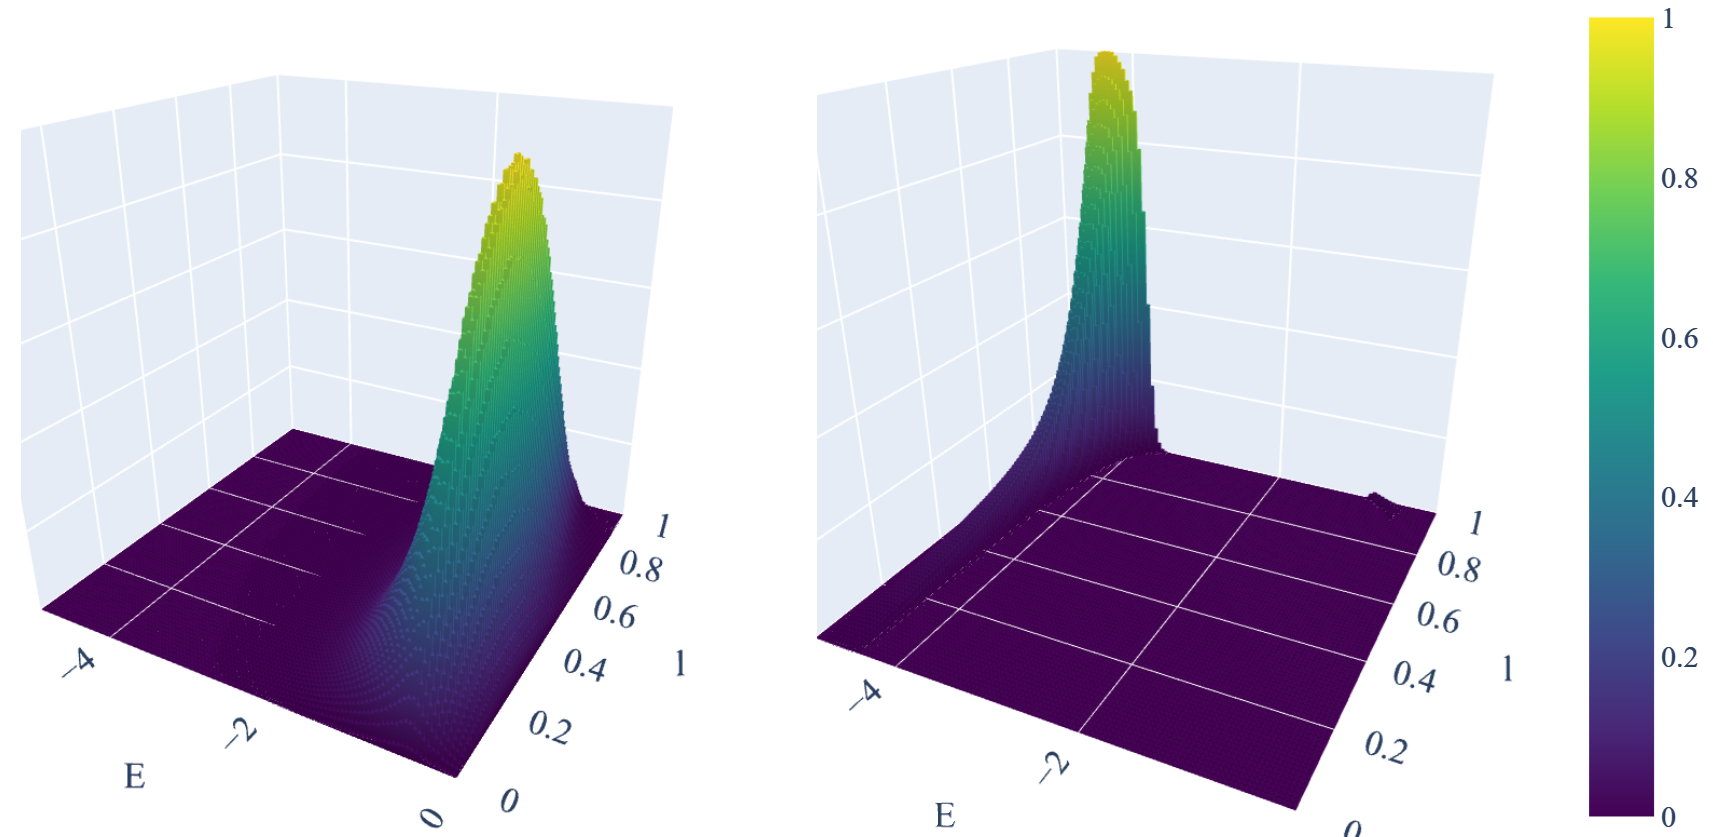
\includegraphics[width=0.7\textwidth]
	{images/Capt100_100.png}
	\caption{Распределение захваченных частиц для $m_{\chi} = 100\, \text{GeV}$, $\delta = 100\, \text{keV}$.}
\end{figure}
	\end{frame}
	
	

	
	\begin{frame}
		\frametitle{Распределение тёмной материи}
		При ненулевом $\delta$ распределение тёмной материи является нетермальным.
\begin{figure}[!h]
	\centering
	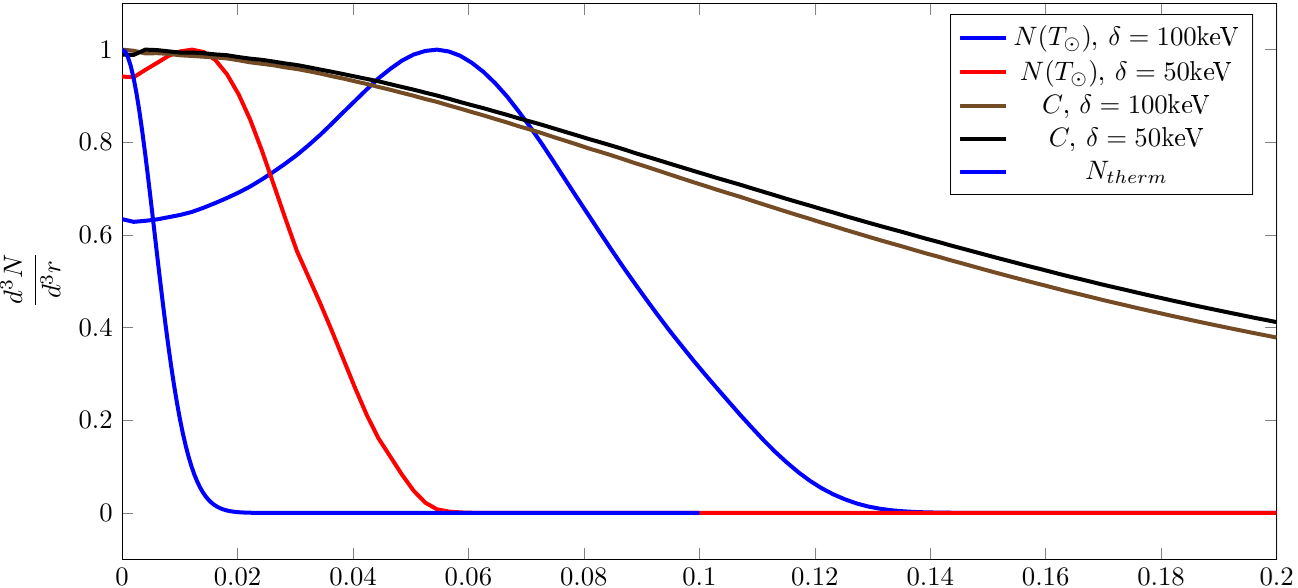
\includegraphics[width=0.8\textwidth]{images/Rdistribs.png}
	\caption{Начальное и конечное радиальное распределение частиц тёмной материи в Солнце $m_{\chi} = 100\text{GeV}$}
	\label{plot:Nrdistrib}
\end{figure}

	\end{frame}
	\begin{frame}
		\frametitle{Захват и аннигилляция}
		\begin{itemize}
	\item Решая численно уравнение эволюции, мы получаем в момент $T_{\odot}$ конечное распределение, откуда находится темп аннигилляции.
\end{itemize}


\begin{figure}[!h]
	\centering
	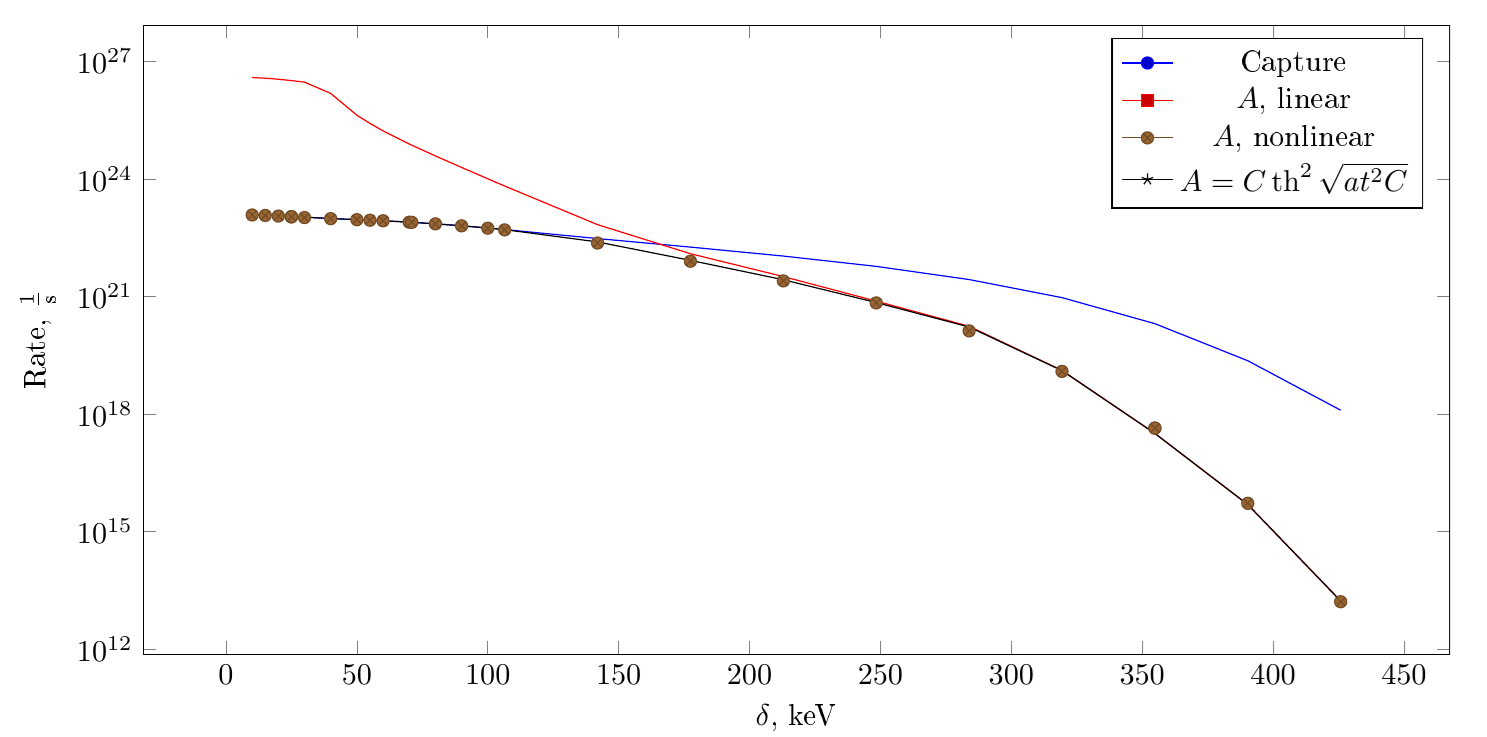
\includegraphics[width=0.8\textwidth]{images/LinearNonLinear.png}
	\caption{Зависимость от $\delta$ захвата и аннигиляции при линейной и нелинейной эволюции для $m_{\chi} = 100\text{GeV}$}
\end{figure}

	\end{frame}
	
	
	\begin{frame}
		\frametitle{Коэффициент аннигилляции}
		\begin{figure}[!h]
	\centering
	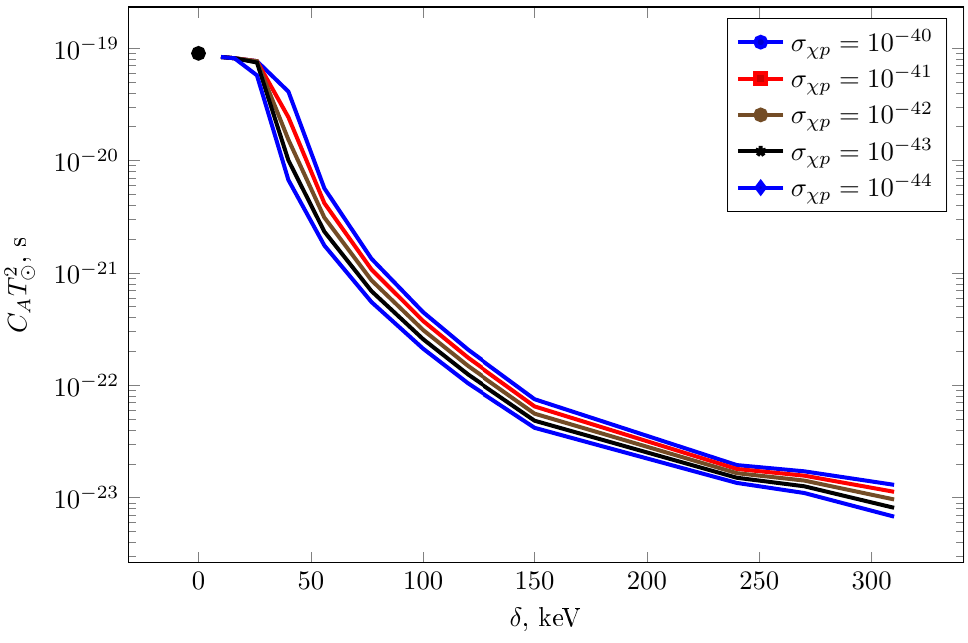
\includegraphics[width=0.7\textwidth]{images/AnnCoeff.png}
	\caption{Коэффициент аннигиляции для $m_{\chi} = 100 \text{GeV}$}
\end{figure}
	\end{frame}
	
	
	\begin{frame}
		\frametitle{Условие равновесия}
		\begin{itemize}
	\item Нам нужно знать при каких $m$ и $\delta$ наступает равновесие между аннигиляцией и захватом а при каких нет.
\end{itemize}


\begin{figure}[!h]
	\centering
	\only<1>{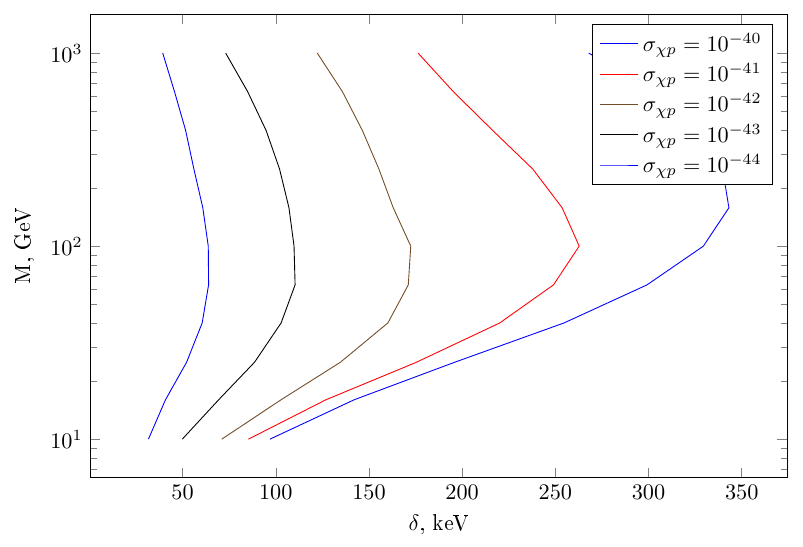
\includegraphics[width=0.65\textwidth]{images/Equilibrium.png}
	\caption{Область параметров $m,\delta$ при которых наступает равновесие между $A$ и $C$ (нераспадающаяся ТМ)}
	}
	\only<2>{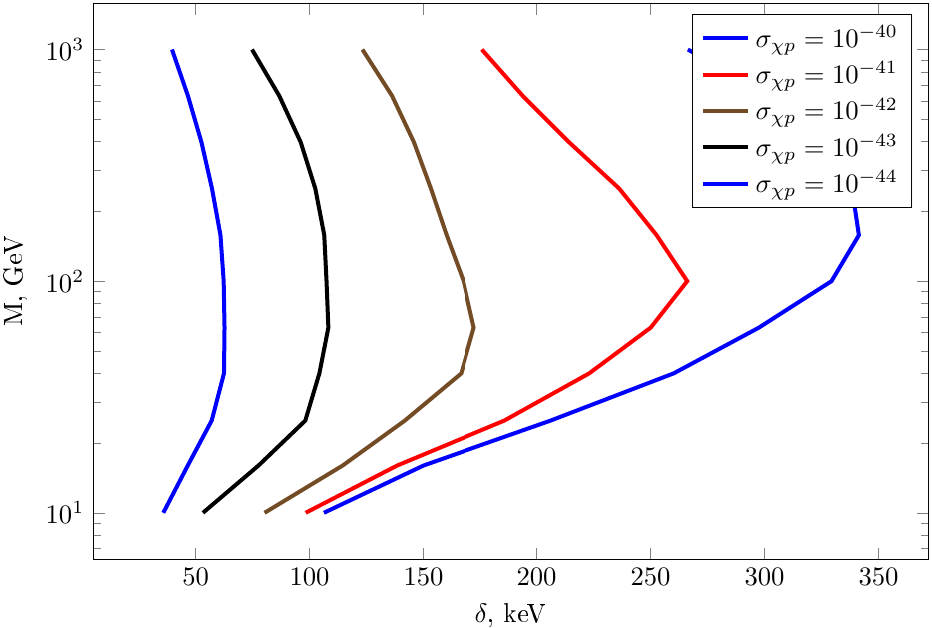
\includegraphics[width=0.65\textwidth]{images/EqFD.png}
	\caption{Область параметров $m,\delta$ при которых наступает равновесие между $A$ и $C$ (распадающаяся ТМ)}
	}
	
\end{figure}

	\end{frame}
	
	\begin{frame}
		\frametitle{Внешняя аннигилляция}
		\begin{itemize}
	\item Часть тёмной материи может аннигилировать снаружи (из-за скопления на траекториях с большим $r$), однако сигнал очень слабый.
\end{itemize}

\begin{figure}[!h]
	\centering
	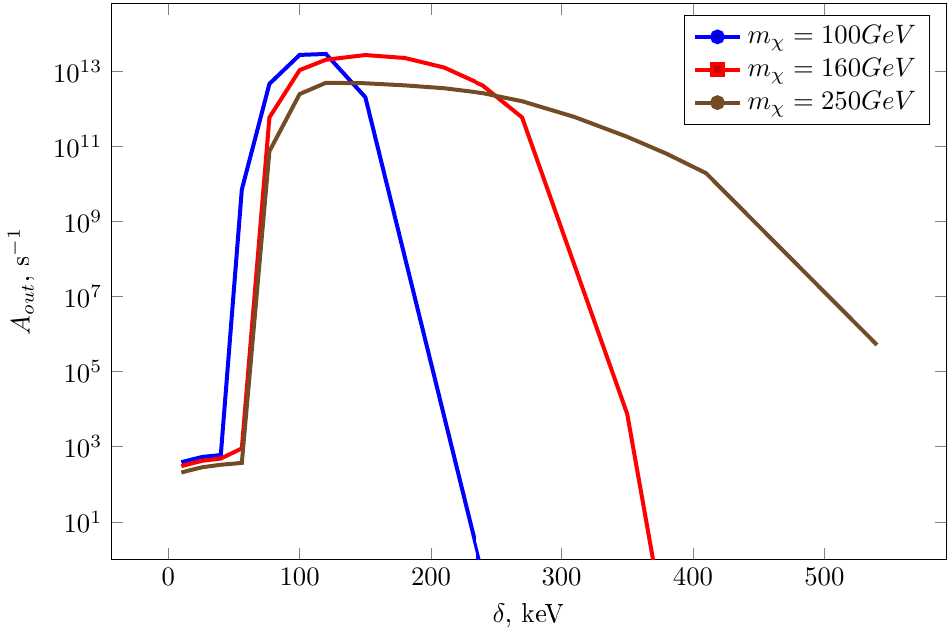
\includegraphics[width=0.65\textwidth]{images/Aout.png}
	\caption{Темп внешней аннигиляции. ($\chi^*$ --- долгоживущая )}
\end{figure}
	\end{frame}
	
	\begin{frame}
		\frametitle{Ограничения}
		\begin{itemize}
	\item ограничить сечение рассеяния можно зная: конечное распределение ($aT_{\odot}^2$), ограничение на темп аннигиляции  $A$ из нейтриного сигнала. 
\end{itemize}
\begin{figure}[!h]
	\centering
	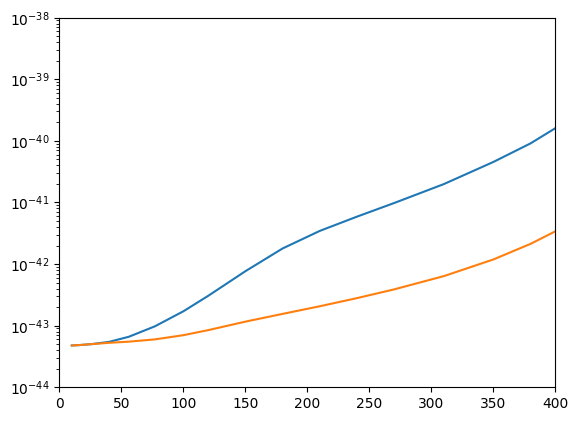
\includegraphics[width=0.65\textwidth]{images/Constrains.png}
	\caption{Пример ограничений из данных IceCube в канале $\chi+\chi \to W^{+} + W^{-}$}
\end{figure}
	\end{frame}
	
	\begin{frame}
		\frametitle{Заключение.}
		\begin{itemize}
	\item Что если включить малое упругое взаимодействие?
	\item Что если включить саморассеяние тёмной материи $\chi + \chi \rightarrow \chi + \chi$?
	
\end{itemize}
	\end{frame}
	\begin{frame}
		\centering
Спасибо за внимание!
	\end{frame}
	
	\begin{frame}
		\frametitle{Сходимость численных схем}
		Упругий случай
\begin{figure}[!h]
	\centering
	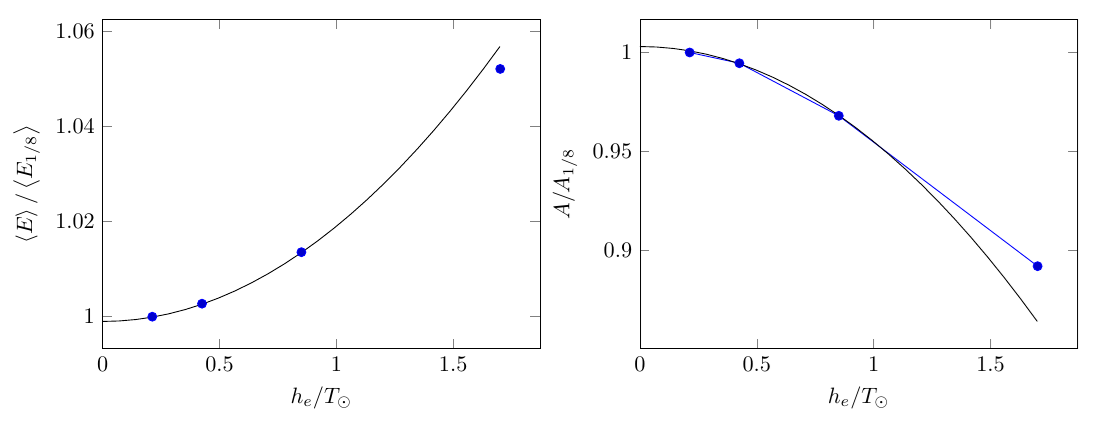
\includegraphics[width=\textwidth]{images/ConvEl.png}
	\caption{Зависимость физических величин (средняя энергия, и темп аннигиляции) от шага решетки $m_{\chi} = 100 \text{GeV}$}
\end{figure}
	\end{frame}
	\begin{frame}
		\frametitle{Сходимость численных схем}
		Неупругий случай
\begin{figure}[!h]
	\centering
	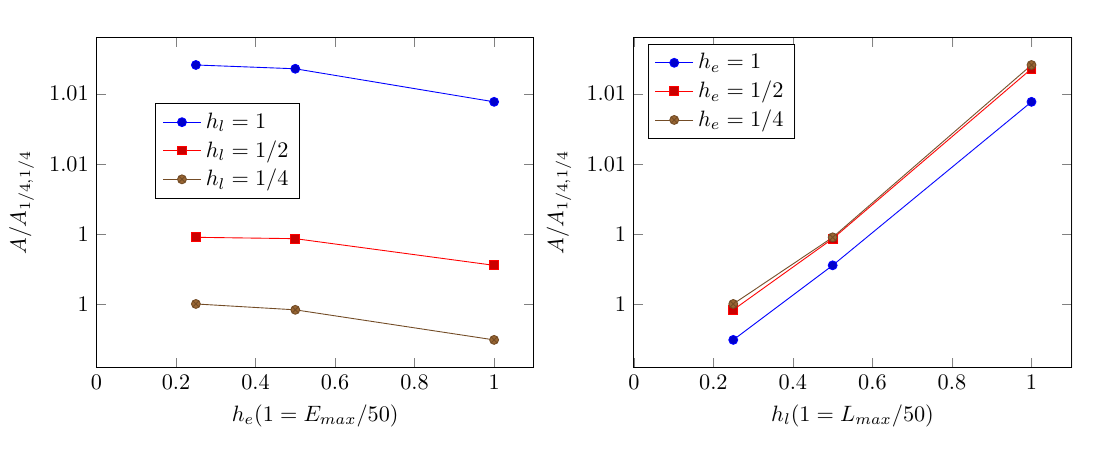
\includegraphics[width=\textwidth]{images/ConvInel.png}
	\caption{Зависимость  темпа аннигиляции от шага решетки по $E$ и $l$ при $m_{\chi} = 100 \text{GeV}$}
\end{figure}
	\end{frame}
\end{document} 

